\documentclass{scrartcl}

\usepackage{graphicx}
\usepackage[siunitx, RPvoltages, european]{circuitikz}

\usepackage{chemformula}
\usepackage[ngerman]{babel}
\usepackage[utf8]{inputenc}
\usepackage{amsmath}
\usepackage{amssymb}
\usepackage[T1]{fontenc}
\usepackage{xcolor}
\usepackage{tikz}
\usepackage[breaklinks=true]{hyperref}
\usepackage[babel,german=quotes]{csquotes}
\usepackage[style=numeric, backend=biber]{biblatex}
\usepackage{listings}
\usepackage{bytefield}
\usepackage{longtable}
\usepackage{sidecap}
\usepackage{wrapfig}
\usepackage{subcaption}
%\usepackage{titlesec}


\graphicspath{ {../../images/} }

\KOMAoptions{parskip=full}

\pdfimageresolution=72


%\titlespacing{\section}{8pt}{12pt plus 4pt minus 2pt}{0pt plus 2pt minus 2pt}
%\titlespacing{\subsection}{4pt}{12pt plus 4pt minus 2pt}{0pt plus 2pt minus 2pt}
%\titlespacing{\subsubsection}{2pt}{12pt plus 4pt minus 2pt}{0pt plus 2pt minus 2pt}


\begin{document}

    \title{Platinencomputer - Langfassung}
    \author{Alexander Wersching und Simon Walter}
    \date{2022}
    \maketitle

    \tableofcontents

    \newpage
    \section{Idee}
    \vspace{-15pt}
    Vor ca. 2 Jahren hatte Alex die Idee: Er wolle einen 8-Bit-Computer bauen.
    Die vor 2 Jahren beim Regionalwettbewerb München-West eingereichte Version eines anderen Teilnehmers hat dann auch mein (Simons) Interesse geweckt.
    \newline
    \vspace{-15pt}
        \begin{wrapfigure}{r}{0.5\textwidth}
        \vspace{-25pt}
        \begin{center}
            \includegraphics[width=0.5\textwidth]{Computer_V01_Overview_01}
        \end{center}
        \vspace{-20pt}
        \end{wrapfigure}
    Ein paar Monate später haben wir uns dann dazu entschieden, tatsächlich einen eigenen 8-Bit-Computer zu bauen und haben auch bald angefangen, erste Versuche auf dem Breadboard zu entwickeln.
    Es gab noch weder eine Möglichkeit diese erste Version automatisch zu betreiben, noch Daten zu schreiben/speichern, oder irgendwie mit der Umgebung zu interagieren, nur 3 Register, 2 Operationen und viele Knöpfe zum Bedienen.


    \section{Nutzen von Platinen}
    \vspace{-15pt}
    \subsection{Warum Platinen?}
    \vspace{-15pt}

        \begin{wrapfigure}{r}{0.4\textwidth}
        \vspace{-40pt}
        \begin{center}
        \includegraphics[width=0.37\textwidth]{Computer_V01_Chaos_07}
        \includegraphics[width=0.37\textwidth,angle=0]{Handy/WP_20210704_20_54_21_Pro}
        \end{center}
        \vspace{-30pt}
        \end{wrapfigure}

    Bald war aber klar, dass ein einfaches Verwenden von flachen Kabeln als Verbindung zwischen den Breadboards, das Kabelgewirr, das wir bei dem Projekt von vor 2 Jahren gesehen haben
    und nach Möglichkeit vermeiden wollten, um ein übersichtlicheres Design zu erreichen, nicht lösen kann.

    Als Alternative für Breadboards haben wir uns für Platinen (PCBs) entschieden.
    Aber weil unser Computer ja nicht mehr wirklich selbst gemacht wäre, wenn wir diese nur professionell ätzen lassen würden,
    wollten wir versuchen - zumindest einen Teil - selbst zu ätzen, auch wenn wir dadurch natürlich auf viele neue Probleme gestoßen sind...


    \newpage

    \subsection{Erste Versuche der Umsetzung}
    \vspace{-15pt}

        \begin{wrapfigure}{l}{0.4\textwidth}
        \vspace{-25pt}
        \begin{center}
        \includegraphics[width=0.4\textwidth,angle=0]{Handy/WP_20210704_20_40_03_Pro} %hier binn ich noch nicht ganz glücklich mit dem Bild
        \end{center}
        \vspace{-20pt}
        \end{wrapfigure}

    Was zu Beginn das Projekt vorangetrieben hat, hat ab diesem Punkt aber natürlich ein Problem dargestellt:
    Das Homeschooling, währenddessen wir natürlich nicht Ätzen können.
    Wir hätten es natürlich zu Hause versuchen können, hatten da aber keine adäquate Ausrüstung v.a. bzgl. Sicherheit.
    Bis wir dann so weit waren, erste Versuche zu machen, war es dann schon Ende 2020.

    Der Herstellungsprozess funktioniert dabei wie folgt:
    \vspace{-10pt}
    \begin{enumerate}
        \item Wir Belichten die Photosensitive Platine mit UV Licht, auf der wir eine mit den Leiterbahnen bedruckte Overheadfolie legen;
        \vspace{-12pt}
        \item Wir legen die Platine - jetzt ohne Folie - in NaOH um die Schutzschicht der Platine an den Belichteten punkten zu lösen;
        \vspace{-12pt}
        \item Als letzten Entwicklungsschritt lösen wir mit FeCl$_3$ das Kupfer ab
        \vspace{-12pt}
        \item Nun werden noch die Entsprechenden Löcher für die THT (Through-hole-technology) Komponenten gebohrt und diese eingelötet
    \end{enumerate}


    \subsection{Design}
    \vspace{-15pt}

        \begin{wrapfigure}{r}{0.65\textwidth}
        \vspace{-40pt}
        \begin{center}
        \includegraphics[width=0.55\textwidth]{3D_Desighn_V21}
        \end{center}
        \caption{Offensichtlich ist das mit unseren aktuell geplanten Modulen: am Boden sitzt eine große Bus-Platine, auf der wir alle Module senkrecht aufstecken.\label{img:design}}
        \vspace{-160pt}
        \end{wrapfigure}

    Nachdem es auch auf geätzten Platinen noch nicht automatisch ordentlich ist und eine derart große Platine für uns nicht machbar gewesen wäre, haben wir uns dann noch ein 3-dimensionales, modulares Design ausgedacht. Dieses ist in \autoref{img:design}


        %\newline
        %\newline
        %\newline

    \newpage
    \section{Anforderungen}
    \vspace{-15pt}
    Im nächsten Lockdown hatten wir dann wieder viel Zeit zu planen, und der geplante Computer wurde immer komplexer.

    \subsection{Daten- und Adresslänge}
    \vspace{-15pt}

    Aus den ursprünglich geplanten 8-Bit wurden 16-Bit-Daten- und Adresslänge:

        \vspace{-5pt}
        \fbox{%
        \parbox{1\textwidth}{

        Die Daten- und Adresslänge besagt, wie viele binäre Ziffern (Bits) für eine Adresse und Daten verwendet werden.\\
        Je mehr Ziffern man verwendet desto größere Zahlen können in einer Operation verarbeitet werden.
            Dabei ist die maximal repräsentierbare Zahl $2^n - 1$ ist, wenn $n$ die Anzahl der Binären Ziffern (= Bits) ist.\\
        Ein $n$ teilbar durch $8$ zu machen, ist dabei relativ angenehm, weil $8$ Bit = $1$ Byte\\
        und Bytes sind nun mal die Grundlage für das meiste in der Informatik,\\
        zudem kommen einige elementare ICs (Integrated Circuits), z.B. Buffer oder Register, immer mit 8 Bits.\\
        \\
        Jedoch gilt, je mehr Bits man verwendet, desto mehr Schaltungen werden benötigt und desto größer der Stromverbrauch, wodurch es für uns relativ schnell unrealistisch aufwendig wird.\\
        \\
        Wir haben uns daher für $16$ Bit entschieden, womit wir
            Zahlen bis zwischen $0$ und $65535$ darstellen können.\\
        Diese Menge ist gerade groß genug, um Zahlen abzubilden, damit die meisten Programme funktionieren können, aber trotzdem noch auf Platinen handhabbar ist.\\

        }%
        }
        \vspace{0pt}

    \newpage
    \subsection{Memory}
    \vspace{-15pt}
    Für Daten und Programme verwenden wir in unserem Computer ein Modul: Memory-Modul

        \begin{wrapfigure}{r}{0.37\textwidth}
        \vspace{-140pt}
        \begin{center}
        \includegraphics[width=0.4\textwidth]{Memory_Map.png}
            \label{img:mem_map}
            \caption{Speicher Aufteilung: Von niederigen zu hohen Addressen in Hexdezimal schreibweiße}
        \end{center}
        \vspace{-20pt}
        \end{wrapfigure}

        \vspace{-5pt}
        \fbox{%
        \parbox{0.6\textwidth}{
        Unser Memory-Modul ist in 65536 einzelne und unabhängige Speicherzellen (jede 16 Bit groß) aufgeteilt. (weil wir genau so viele Adressen in unseren 16 Bit speichen können)\\
        Der Computer kann damit auf $65536 \text{ Words}$ oder $131072 \text{ Bytes}$ ($= 128 \text{ kib}$) direkt zugreifen.\\
        Die Größe messen wir in Words (w) oder in Kilowords (kiw), wobei $1 \text{ Word} = 2 \text{ Bytes} = 16 \text{ Bit}$ sind.\\
        \\
        Memory wird dabei über LD- und STR-Instruktionen gesteuert.\\
        Die LD-Instruktion kopiert einen Wert aus Memory und schreibt ihn in das Ziel-Register, während STR an der angegebenen Adresse den Wert mit dem Wert des Quellen-Register überschreibt.\\

        }
        }
        \vspace{0pt}

    Um aber noch mehr Speicher zu nutzen und das später erwähnte Berechtigungssystem möglichst leicht umsetzen zu können, haben wir noch Banken hinzugefügt:

        \vspace{-5pt}
        \fbox{%
        \parbox{1\textwidth}{
        Banken sind externe Memory Module, die eingesteckt werden können.
        Alle Banken sind gleich groß ($16\text{ kiw} = 32\text{ kib}$) und der Computer unterstützt maximal $65536$ unterschiedliche Banken.
        Jede Bank hat dabei eine ID (BID), die von $0$ bis $65535$ reicht.

        Der Computer hat zwei Bank-Slots (Slot 1 \texttt{0x8000 - 0xbfff} und Slot 2 \texttt{0xc000 - 0xffff}), auf den jeweils eine der Banken gelegt werden kann.
        \newline
        \newline
        Bank-Slot $1$ ist dafür gedacht, dass jeder Prozess dort in seiner eigenen Bank lebt, sodass in dem Prozess absolute Memory Adressen verwendet werden können, weil das Programm immer an der gleichen Stelle liegt.
        Außerdem wird in der Bank auch der Stack des jeweiligen Prozesses gespeichert, sodass dieser von anderen Prozessen nicht überschrieben werden kann.

        Bank-Slot $2$ dient als potentieller zusätzliche Speicher des Prozesses, oder als allgemeiner Speicherort, um zwischen den Prozessen Daten zu übermitteln.

        }%
        }

    \subsection{ROM}
    Um den Computer komplett unabhängig funktionsfähig machen zu können, haben wir uns dann überlegt einen Teil des RAMs (\texttt{0x0000} - \texttt{0xffff}) durch ROM zu ersetzen, um automatisch Programme von einem externen Speichermedium laden zu können. Zusehen in \autoref{img:mem_map}

    \subsection{Instruktionen}
    \vspace{-15pt}
    Um die neuen Möglichkeiten durch 16-Bit auch sinnvoll nutzen zu können, haben wir dann noch viele Logikoperationen und komplexere konditionale Jumps hinzu gefügt:
    Der Computer soll die Grundoperationen: Addition (ADD), Subtraktion (SUB), Multiplikation (MUL), Division (DIV),
    so wie die bitweisen Operationen: Exklusives Oder (XOR), Und (AND), Nicht (NOT) und Oder (OR) beherrschen.

    Der Computer besitzt zudem folgende Instruktion um mit Memory zu interagieren: Laden (LD), Speicher (STR), Bank 1 und
    Bank 2 wechseln (BNK1 und BNK2) und folgende Instruktion um mit dem Hardware Stack zu interagieren: push (PUSH), pop
    (POP), Funktionsaufruf (CALL) und Funktionsrückgabe (RET).

    Zudem die folgenden IO-Instruktionen: Instruktion Send (IOUT), Daten Senden (DOUT), Daten lesen (DIN), IO-Gerät Aktivieren (AIO) und IO-Gerät Deaktivieren

    Aber auch noch folgende Instruktion um Interrupts zu verwalten: Software Interrupt auslösen (INT), Modus des Timers 1 und 2 setzten (TM1/TM2) und die Stop Werte des Timers 1 und 2 setzten (SSTL1/SSTL2/SSTH1/SSTH2)

    Insgesamt hat unser Computer damit folgende Instruktionen: \autoref{table:instructions}

    \vspace{-15pt}
    \begin{center}
        \begin{longtable}{l | l l l l | l}
            \kill
            \caption{\label{table:instructions}Instruktions-Satz}
            \endhead
            Ins-ID & Name & op1 & op2 & op3 & Beschreibung \\
            \hline
            \texttt{0x00} & NOP  &  &  &  & Kein Effekt  \\
            \hline
            \texttt{0x01} & MOV  & reg &  & reg/c & op1 $=$ op3\\
            \texttt{0x02} & ADD  & reg & reg & reg/c & op1 $=$ op2 $+$ op3 \\
            \texttt{0x03} & SUB  & reg & reg & reg/c & op1 $=$ op2 $-$ op3 \\
            \texttt{0x04} & MUL? & reg & reg & reg/c & op1 $=$ op2 $*$ op3 \\
            \texttt{0x05} & MULOF& reg & reg & reg/c & op1 $=$ Overflow op2 $*$ op3 \\
            \texttt{0x05} & DIV? & reg & reg & reg/c & op1 $=$ op2 $/$ op3 \\
            \texttt{0x06} & XOR  & reg & reg & reg/c & op1 $=$ op2 $\oplus$ op3 \\
            \texttt{0x07} & AND  & reg & reg & reg/c & op1 $=$ op2 $\land$ op3 \\
            \texttt{0x08} & OR   & reg & reg & reg/c & op1 $=$ op2 $\lor$ op3 \\
            \texttt{0x09} & NOT  & reg &  & reg/c & op1 $=$ $\lnot$op3 \\
            \hline
            \texttt{0x0a} & STR  &  & reg & reg/c & memory[op3] = op2 \\
            \texttt{0x0b} & LD   & reg & reg & reg/c & op1 = memory[op2 + op3] \\
            \texttt{0x0c} & BNK1 &  &  & reg/c & Setzt BID für Bank-Slot1 \\
            \texttt{0x0d} & BNK2 &  &  & reg/c & Setzt BID für Bank-Slot2 \\
            \hline
            \texttt{0x0e} & PUSH &  &  & reg/c & SP--; memory[SP] = op1 \\
            \texttt{0x0f} & POP  &  &  & reg & op3 = memory[SP]; SP++ \\
            \texttt{0x10} & CALL &  &  & reg/c & \vtop{
				\hbox{\strut memory[SP] = IP; SP++;}
				\hbox{\strut IP = op3}} \\
            \texttt{0x11} & RET  &  &  &  & IP = memory[SP]; SP++ \\
            \hline
            \texttt{0x12} & TEST & reg &  & reg/c & Vergleicht op1 und op3 \\
            \texttt{0x13} & ME   & reg &  & reg/c & op1 = op3 if E \\
            \texttt{0x14} & MG   & reg &  & reg/c & op1 = op3 if G \\
            \texttt{0x15} & ML   & reg &  & reg/c & op1 = op3 if L \\
            \texttt{0x18} & MOFadd  & reg &  & reg/c & op1 = op3 if O \\
            \texttt{0x19} & MOFsub  & reg &  & reg/c & op1 = op3 if O \\
            \hline
            \texttt{0x1a} & IOUT & reg &  & reg/c & IIO[op1] = op3/c \\
            \texttt{0x1b} & DOUT & reg &  & reg/c & DIO[op1] = op3/c \\
            \texttt{0x1c} & DIN  & reg &  & reg & op3 = DIO[op1] \\
            \texttt{0x1d} & AIO  & reg &  &  & Aktiviert IO[op1] \\
            \texttt{0x1e} & DIO  & reg &  &  & Deaktivieren IO[op1] \\
            \hline
            \texttt{0x1f} & INT  & & & & Löst einen Interrupt aus \\
            \texttt{0x20} & TM1  & & & reg/c & Modi Timer1 = op3 \\
            \texttt{0x21} & TM2  & & & reg/c & Modi Timer2 = op3 \\
            \texttt{0x22} & SSTL1 & & & reg/c & erster Stop Timer1 = op3 \\
            \texttt{0x23} & SSTL2 & & & reg/c & zweiter Stop Timer2 = op3 \\
            \texttt{0x24} & SSTH1 & & & reg/c & erster Stop Timer1 = op3 \\
            \texttt{0x25} & SSTH2 & & & reg/c & zweiter Stop Timer2 = op3 \\
            \texttt{0x26} & CFL  & reg & & & op1 = erster Clock Freq \\
            \texttt{0x27} & CFH  & reg & & & op1 = zweiter Clock Freq
        \end{longtable}
    \end{center}

    \subsection{IO-Ports}
    \vspace{-15pt}
    Dazu hat sich die Idee von komplexer IO-Interaktion mit dem Computer ergeben:
    universelle Ports zum Anschließen von Festplatten, Sensoren, einfachen Tastaturen, LCD-Displays oder einer Grafikkarte.

        \vspace{-5pt}
        \fbox{%
        \parbox{1\textwidth}{
        Die theoretisch 65536 Anschlüsse, wobei jedem eine Anschluss-ID zugewiesen ist, kommunizieren mit IO-Geräten über 4 Kommandos,
            die als 4 separate Pins zwischen dem Controller und dem Gerät umgesetzt sind:

        1. Einen Befehl an das IO-Gerät schicken (auf Programm-Ebene);

        2. Daten zu einem vorherigen Befehl an das Gerät schreiben;

        3. Die Anfrage des IO-Gerätes, Daten an den Computer zurück zu schreiben, was bei diesem normalerweise einen Interrupt auslöst;

        4. Bestätigen des Computers, das das Externe Gerät schreiben darf;

        }%
        }

    \subsection{Supervisor-/Usermode}
    \vspace{-15pt}



        Er kann dabei in zwei Modi operieren: dem Supervisormode und Usermode.
        Im Supervisormode kann der Computer alle Funktion ohne Einschränkungen nutzen.
        Im Usermode hingegen ist der Computer in einigen Funktion eingeschränkt.
        Folgendes kann der Computer im Usermode \emph{nicht} machen:

        \begin{itemize}
            \item Setzen der SUP Flagge
            \item Änderung der OINT Flagge
            \item Lesen und/oder schreiben im Bereich von \texttt{0x0000} - \texttt{0x7fff}
            \item Änderung der Banken
            \item Die Modifikation der IO-Berechtigungsliste
            \item Zugriff auf IO-Geräte, welche nicht in der Berechtigungsliste gespeichert sind (siehe \autoref{section:persmissionIO})
        \end{itemize}

    Wir haben uns entschieden eine Art Berechtigungssystem in der Computer einzubauen.
    Eine Rechner der nur einfache Programm ausführt um zu Beispiel eine LED oder ein LCD-Display zu steueren, wie es z.B. ein ESP32 oder ein ATMega328p macht, ist so ein System nicht nötig.
    Wir hatten jedoch vor mit unserem Computer die Möglichkeit zu schaffen ein Betriebssystem ähnliches Programm (Supervisor) laufen zulassen.

    Hierfür hat man ein mal den Supervisor, der bei Start des Computer anfängt zulaufen und Programme, welche im Usermode ausgeführt werden, sogenannte Prozesse, lädt.
    Dabei sieht ein typischer Programmablauf ist dabei in gezeigt.

    Wichtig ist, das sobald ein Prozess beendet wurde, der Supervisor an dieser Stelle wieder anfängt und den nächsten Prozess startet.

    Ein Prozess kann auch Funktionen des Supervisor nutzten über Software Interrupts, da bei einem Interrupt, der Computer in den Supervisormode wechselt.
    So kann der Prozess, bevor er den Interrupt auslegt, ein oder mehrere Register nutzten um Werte an den Supervisor zu übergeben.
    z.B. kann er eine Register nutzten um dem Supervisor zu sagen was er tun soll, z.B. dem Prozess zugang zu einem IO-Gerät zugeben oder etwas in eine Datei zuschreiben.
    Diese Art von Kommunikation werden auch System-Calls genannt und sind die Basis für jedes moderne Betriebssystems.

    Ein solcher Supervisor kann sehr mächtig sein:

    \begin{enumerate}
        \item Abstraktion der Hardware: Oft ist die IO-Configuration von Setup zu Setup sehr verschieden. Ein Prozess welcher IO-Geräte nutzen möchte hat oft den Nachteil dass es für ein bestimmtes Hardware setup geschrieben wurde. So z.B. ein Prozess der Daten einer SD-Karte ausließt und diese anzeigt. Wenn man jedoch jetzt eine Floppy-Laufwerk anschließt, so kann man das Prozess zum Auslesen nicht verwenden, da es nur die Kommuntiation mit einer SD-Karte kennt. Der Supervisor könnte an dieser Stelle ein Interface über System-Calls bieten welches unabhänige von dem Gerät ist. So im diesem Beispiel ein Dateisystem, auf welches Prozesse zugreifen können. Somit übernimmt der Supervisor die Kommuntiation mit der Hardware.

        \item Teilung der Rechenzeit: Der Computer so viele Features er doch hat, ist stark limitiert vor allem was Rechengeschwindigkeit betrifft. Wenn man nun mehrer Programm hat, welche ausgeführt werden sollen, so wäre es natürlich sehr einfach sie der Reihe nach auszuführen. Jedoch gibt es bessere Wege, so z.B. das der Computer jedem Prozess nur eine bestimmte Rechenzeit gibt und dann den nächsten Prozess ausführt. Das kann erreicht werden durch folgenden Ablauf: Der Supervisor stellt vor dem ausführen des Prozesse eine Timed-Interrupt. Dann übergibt der Supervisor den Computer dem Prozess, welcher dann seine Programm ausführt. Dies machter bis der Timed-Interrupt ausgelöst wird und der Computer wieder in den Supervisormode wechselt. Dieser speichert nun alle Register und Banken Configuration des Prozesse und übergibt einem anderen Prozesse den Computer. Wenn nun ein schon angefanger Prozess wieder gestarted werden soll läd der Supervisor wieder die Register und Banken des Prozesses und übergibt die Außführung wieder an den Prozess. Somit kann der Computer zwischen Prozessen hin und herschallten, was die Illusion gibt, das der Computer diese gleichzeitig ausführt.

        \item Isolation von Prozessen: Programme sind meist nicht perfekt. Vor allem sowas wie Bufferoverflows und andere Fehler dieser Art treten in Low-Level Systeme gerne auf. Aus diesem Grund ist es wichtig Prozesse von einander zu isolieren. Nehmen wir an Prozess A hat ein Fehler welcher dafür sorgt das er den gesammten RAM anfängt voll zuschreiben. Um jetzt Prozess A daran zuhinern Prozess B zu überschreiben, ist es dem Prozess A nicht gestattet auf den Arbeitsspeicher von Prozess B zuzugreifen. Nur der Supervisor kann zwischen den Prozessen wechseln
    \end{enumerate}

    Wenn man so etwas will kann dass auch auf einem ATMega328p gemacht werden, jedoch nicht ohne massive Leistungsverluste.
    Wenn so ein Berechtigungssystem jedoch direkt in die Hardware des Computers einfließt sorgt das für eine viel effektiveren Computer.

    Wenn man tatsächliche nur Programme schreiben will welche ''nur'' ein LED oder LCD-Display steuern soll, kann man das mit unserem Computer auch machen, indem man einfach dieses Programm im Supervisor laufen lässt.

    \section{Tests}
    \subsection{Breadboard-Test}
        %\begin{wrapfigure}{r}{0.65\textwidth}
        %\vspace{-40pt}
        %\begin{center}
        %\includegraphics[width=0.55\textwidth]{Perspektive_P}
        %\end{center}
        %\vspace{-50pt}
        %\end{wrapfigure}
    Zwischendurch haben wir dann für die Einladung zu der lokalen Veranstaltung
    $"$Perspektive P$"$ am 15.07.2021 wieder einen unvollständigen Prototyp auf dem Breadboard gebaut.

    \subsection{Geschwindigkeit}
    \vspace{-15pt}
        \begin{wrapfigure}{r}{0.4\textwidth}
        \vspace{-20pt}
        \begin{center}
        \includegraphics[width=0.4\textwidth]{20211208_200750_}
        \caption{Messaufbau\label{img:PD_Messurement}}
        \end{center}
        \vspace{-20pt}
        \end{wrapfigure}

    Um zu errechnen, wie schnell wir den Computer maximal laufen lassen können, ohne fehlerhafte Ergebnisse zu erhalten, haben wir den ''Propagation-Delay'' gemessen.
    Der ''Propergation-Delay'' ist die Zeit, bis der Chip den Output liefert, den der laut der Eingabe haben müsste. Wir haben diese Messungen bei einigen unserer wichtigsten Komponent durch geführt.
    Die meisten Chips, die wir jetzt vorhaben zu verwenden, haben eine Properagtion-Delay von zwischen $10$ und $20$ ns wie z.B. bei NAND, AND oder OR-Gatteren.
    Allerdings haben wir bei den einigen Versionen, die wir getestet haben, teilweise weitaus höhere Werte bis zu $150$ ns gemessen.
    Dies ist an sich noch nicht so schlecht, aber wenn wir damit rechnen, dass wir Reihen von bis zu $40$ Chips verwenden, limitiert das die Geschwindigkeit schon sehr. Der Messaufbau den wir verwendet haben ist dabei in \autoref{img:PD_Messurement} zusehen. Die Ergebnisse einer solchen Messung können in \autoref{img:res_PD} eingesehen werden.

    \begin{figure}
        \includegraphics[width=0.9\textwidth]{NANDs_Result_Rising}
        \caption{Messergebnisse der Propergation-Delay Messung von drei Quod-NAND-Gattern in Verschieden Ausführungen (CD4096BE, SN74HC00, SN74HCT00)\label{img:res_PD}}
    \end{figure}

    \newpage
    \subsection{Funktionsweise der Chips}
    \vspace{-15pt}
    Wir wollen als Basis für unseren Computer ja Chips kaufen, aber wie funktionieren die eigentlich?
    Wir haben also versucht den Aufbau herauszufinden, indem wir einfach einen geöffnet haben, wobei $"$einfach$"$ nicht so ganz stimmt, weil die Hülle aus Epoxidharz besteht, was sich fast nicht auflösen lässt.
    Also mussten wir mechanisch abtragen, also Schleifen.
    Leider haben wir es damit nie geschafft das gesamte Silizium/die Verbindungsbahnen frei zu legen, sodass wir keinen Schaltplan erstellen könnten,
    es gab uns aber trotzdem eine beeindruckende persönliche Einsicht:


        \begin{figure}[h]
        \begin{subfigure}[b]{0.3\textwidth}
            \includegraphics[width=\textwidth]{WP1_09}
            \end{subfigure}
        ~
        \begin{subfigure}[b]{0.3\textwidth}
            \includegraphics[width=\textwidth]{WP_20211029_143251_}
            \end{subfigure}
        ~
        \begin{subfigure}[b]{0.3\textwidth}
            \includegraphics[width=\textwidth]{WP_20210917_16_56_15}
            \end{subfigure}
        \end{figure}

    \newpage
    \section{Umsetzung}
    \vspace{-15pt}
    \subsection{Programmierung}
    \vspace{-15pt}

        \begin{wrapfigure}{r}{0.6\textwidth}
        \vspace{-30pt}
        \begin{center}
        \includegraphics[width=0.6\textwidth]{ROM_Programmer_Manual_01}
        \end{center}
        \vspace{-20pt}
        \end{wrapfigure}

    Um den ROM-Chip zu programmieren haben wir zwar mal kurz ein bisschen manuell über Schalter programmiert, aber nachdem das offensichtlich zu lange brauchen würde haben wir dann einen Arduino (um genau zu sein, einen ESP32) programmiert und an die pins des ROM-Chips angeschlossen.
    Der Arduino bekommt die zu schreibenden bits wiederum aus einem Python-Programm, das den Assembler in Maschinensprache (eine binary Datei) umwandelt.

    \includegraphics[width=0.8\textwidth]{assembler_code}

    \newpage
    \subsection{Weitere Tests zum Ätzen}
    \vspace{-15pt}
    Im Schuljahr 2021-2022 haben wir dann wieder weitere Tests zum Ätzen - diesmal sowohl erfolgreicher, als auch besser dokumentiert, um die optimalen Belichtungs- und Ätzzeiten zu finden.
    Diese sind in der nebenstehenden Tabelle aufgelistet.
    \newline
    \vspace{-5pt}
    \includegraphics[width=0.9\textwidth]{aetzen_tabelle}

    Es hat sich folgender Ablauf funktioniert nach unseren Test am besten: Ein Belichtungszeit von $20$ bis $30$ min, mit den Konzentrationswerten von
    c(\ch{NaOH}) $= 0.015 \text{g/ml}$, c(\ch{FeCl3}) $= 0.8 \text{g/ml}$. Dabei ist zubachten, dass das Entwickeln und Ätzen unter Bewegung statfinden muss.

    \subsection{Spezifikation}
    \vspace{-15pt}
    Gleichzeitig haben wir auch angefangen unsere erste vollständige Version der Spezifikation zu schreiben siehe: \href{https://www.mediafire.com/file/9iz9wlpiuwhr1ln/HandBuch.pdf/file}{Handbuch.pdf}

    \newpage
    \subsection{Nutzung eines zwei Busses}
    \vspace{-15pt}
    Um Memory innerhalb eines Clock-Zyklus zu beschreiben, muss diesem sowohl eine 16-Bit-Adresse als auch den 16-Bit-Daten-Wert übermittelt werden.
    Damit diese beiden Daten parallel übermittelt werden können brauchen wir also 2*16 Bit.
    Wir hätten dafür natürlich auch irgendwelche Kabel verlegen können, aber wir wollen in unserem System die Daten immer auf dem Bus transportieren, damit diese auch von anderen Modulen gelesen werden könnten.
    Die Adresse muss im Anwendungsfall des Stacks vor Benutzung um eins erhöht oder verringert werden, was in unserem System durch die ALU erfolt, wobei diese ihre Daten nur auf den Bus auseben kann.
    Dabei hat sich ein Aufbau wie in \autoref{img:schematic_all} ergeben.

    \begin{figure}
        \vspace{-15pt}
    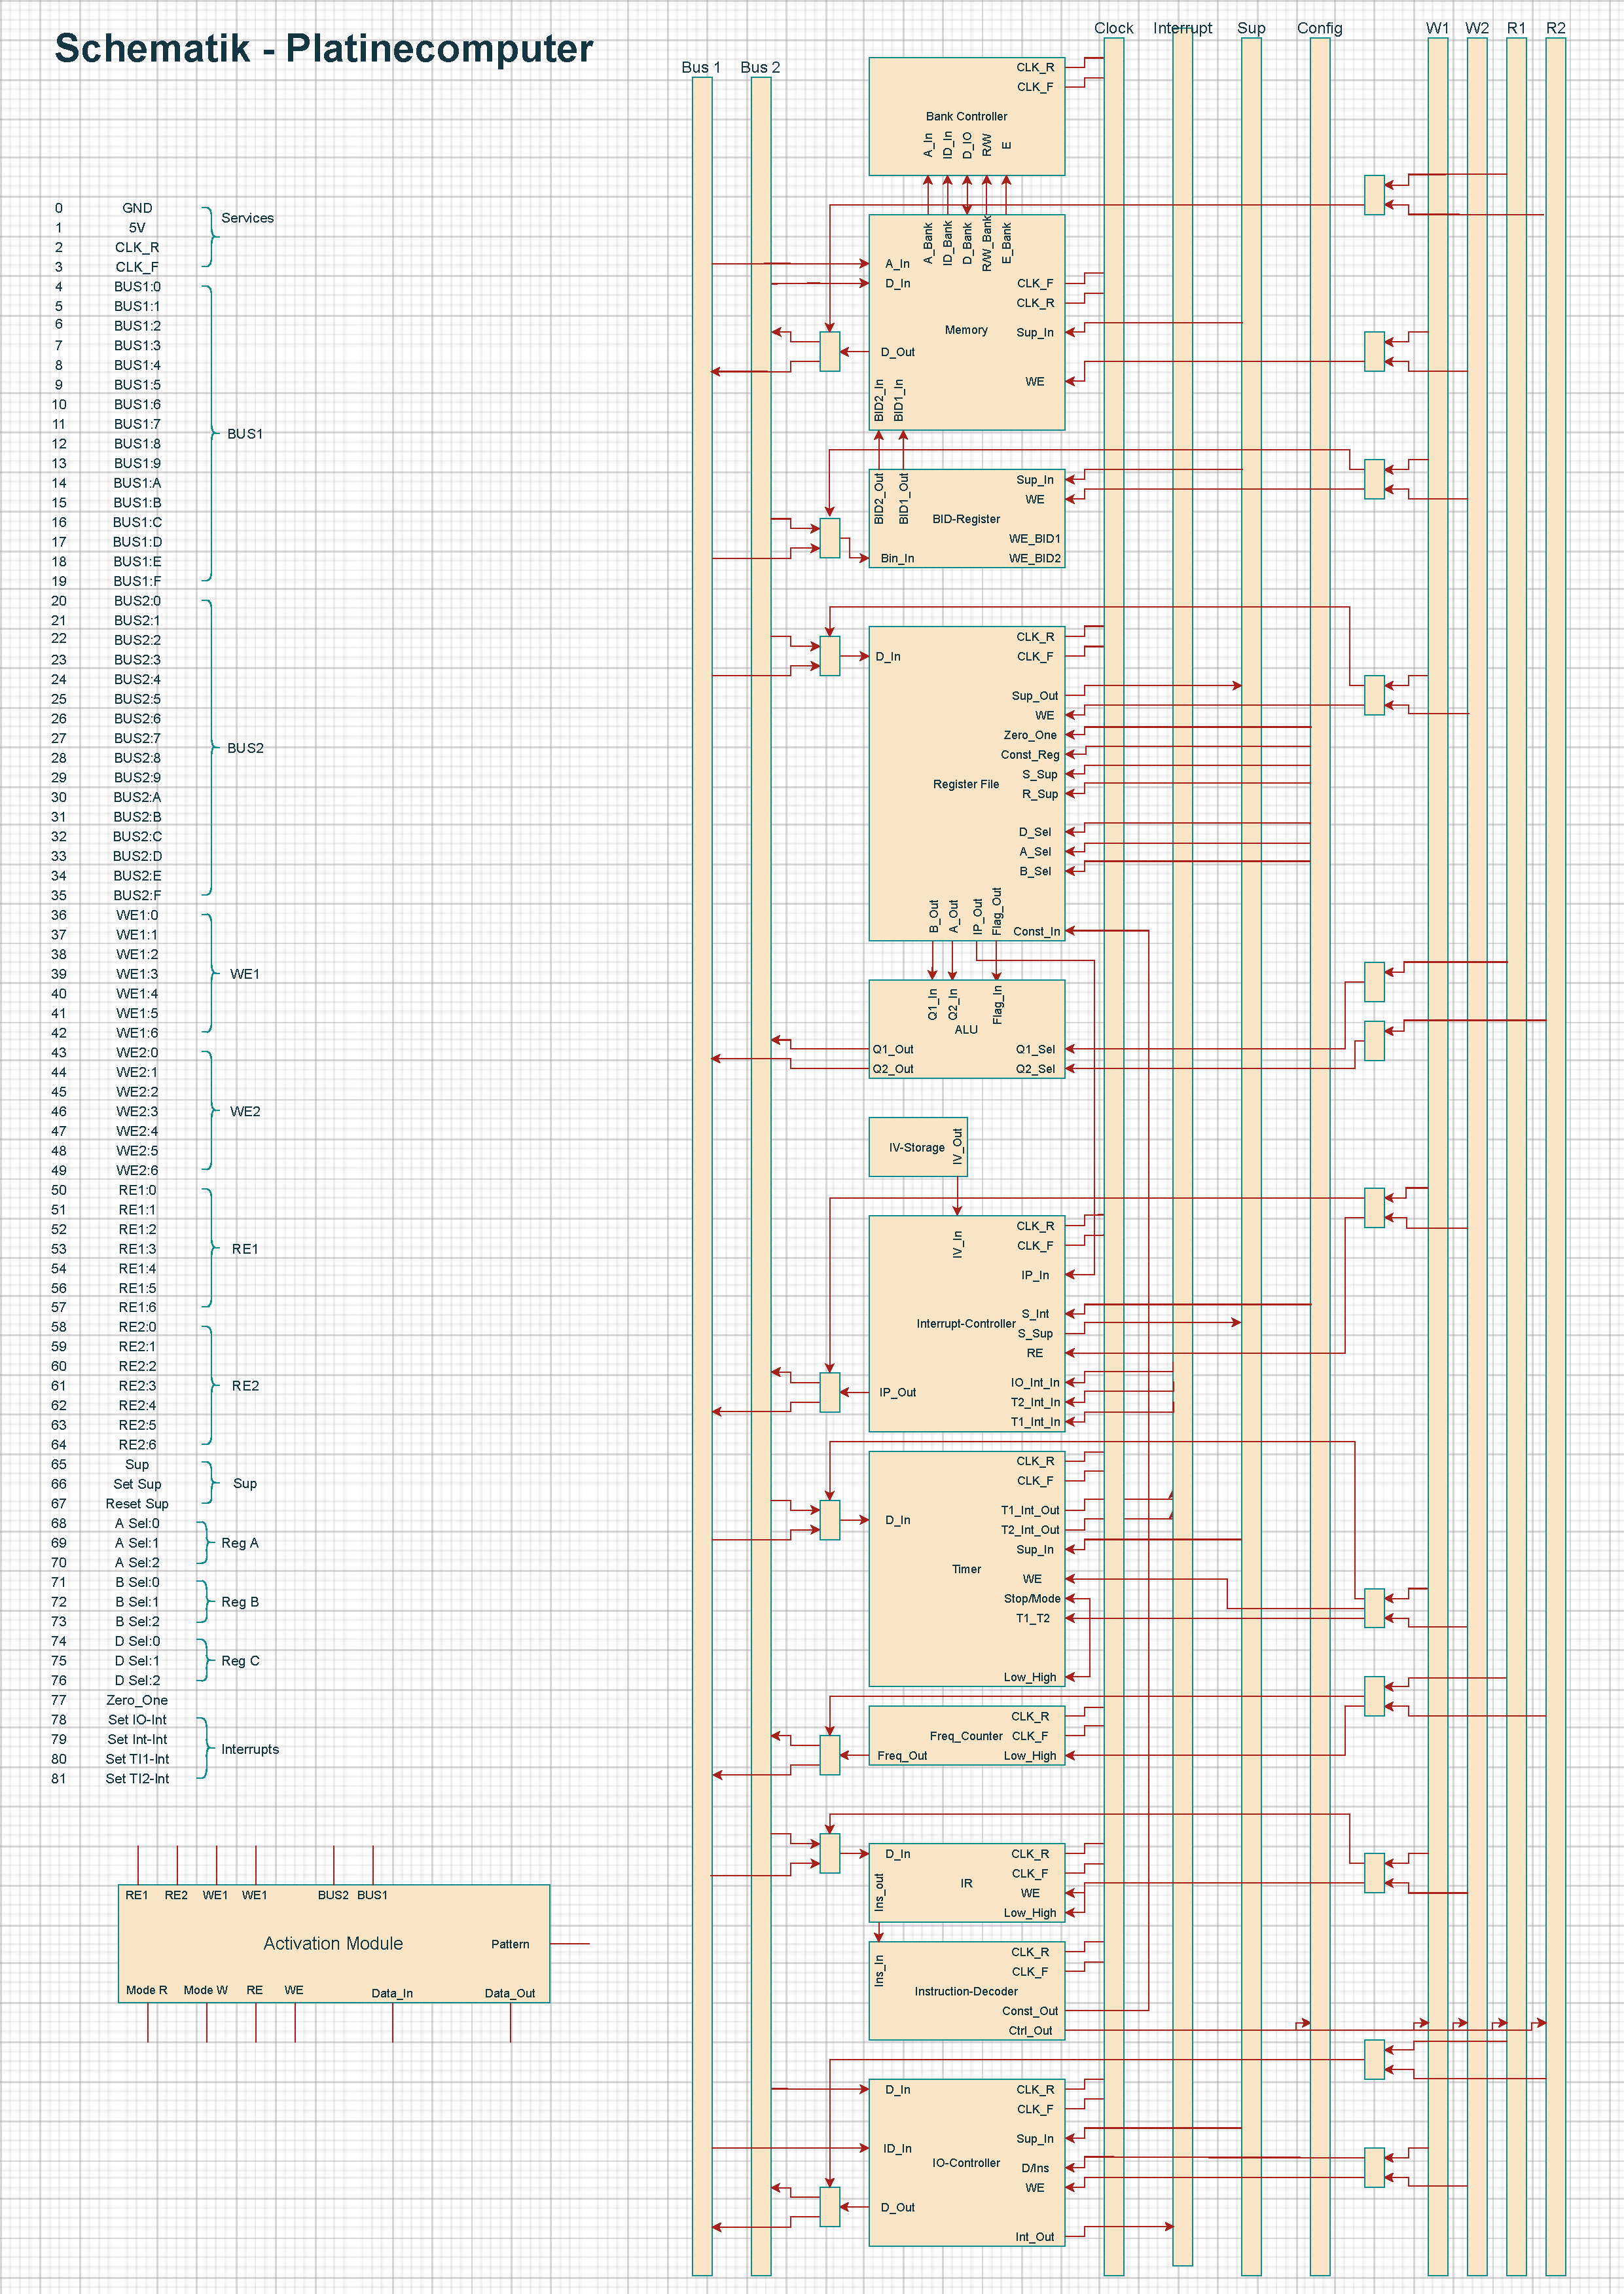
\includegraphics[width=0.612\textwidth]{arch.drawio}
        \caption{Schematischer Aufbau des Computers\label{img:schematic_all}}
        \vspace{-15pt}
    \end{figure}

    \newpage
    \subsection{Design der Schaltungen}
    \vspace{-15pt}

        \begin{wrapfigure}{r}{0.7\textwidth}
        \vspace{-20pt}
        \begin{center}
        \includegraphics[width=0.65\textwidth]{kicad_schematic}
        \includegraphics[width=0.65\textwidth]{kicad_pcb}
        \end{center}
        \vspace{-20pt}
        \end{wrapfigure}
    Zum Designen haben wir uns schlussendlich darauf festgelegt, dass wir die Schaltungen zuerst in dem Logiksimulationsprogramm Logisim erstellen,
    und danach den Plan noch einmal als ätzbaren Schaltplan erstellen, wobei wir hierfür kein wirklich zufriedenstellendes Produkt finden konnten.
    Schließlich haben wir uns vor allem wegen der Einfachheit es zu bekommen und Installieren für KiCad entschieden, was uns allerdings ziemlich viel Frust beschert hat.


\end{document}
